\documentclass[border=8pt]{standalone}
\usepackage{amsmath,amssymb}
\usepackage{tikz}
\usetikzlibrary{arrows.meta,backgrounds,calc,decorations.pathreplacing,fit,matrix,positioning}

\definecolor{paperpink}{HTML}{F4DADA}
\definecolor{paperlavender}{HTML}{E9E4F1}
\definecolor{papergreen}{HTML}{DDECDD}
\definecolor{paperyellow}{HTML}{F5F2C8}
\definecolor{paperpeach}{HTML}{FBEBD6}
\definecolor{paperblue}{HTML}{E2ECF4}
\definecolor{ink}{HTML}{252525}
\definecolor{rulegray}{HTML}{8B9298}
\definecolor{cachegray}{HTML}{ECEFF1}
\definecolor{newblue}{HTML}{B9D7EA}
\definecolor{prefill}{HTML}{DDECDD}
\definecolor{decode}{HTML}{FBEBD6}

\begin{document}
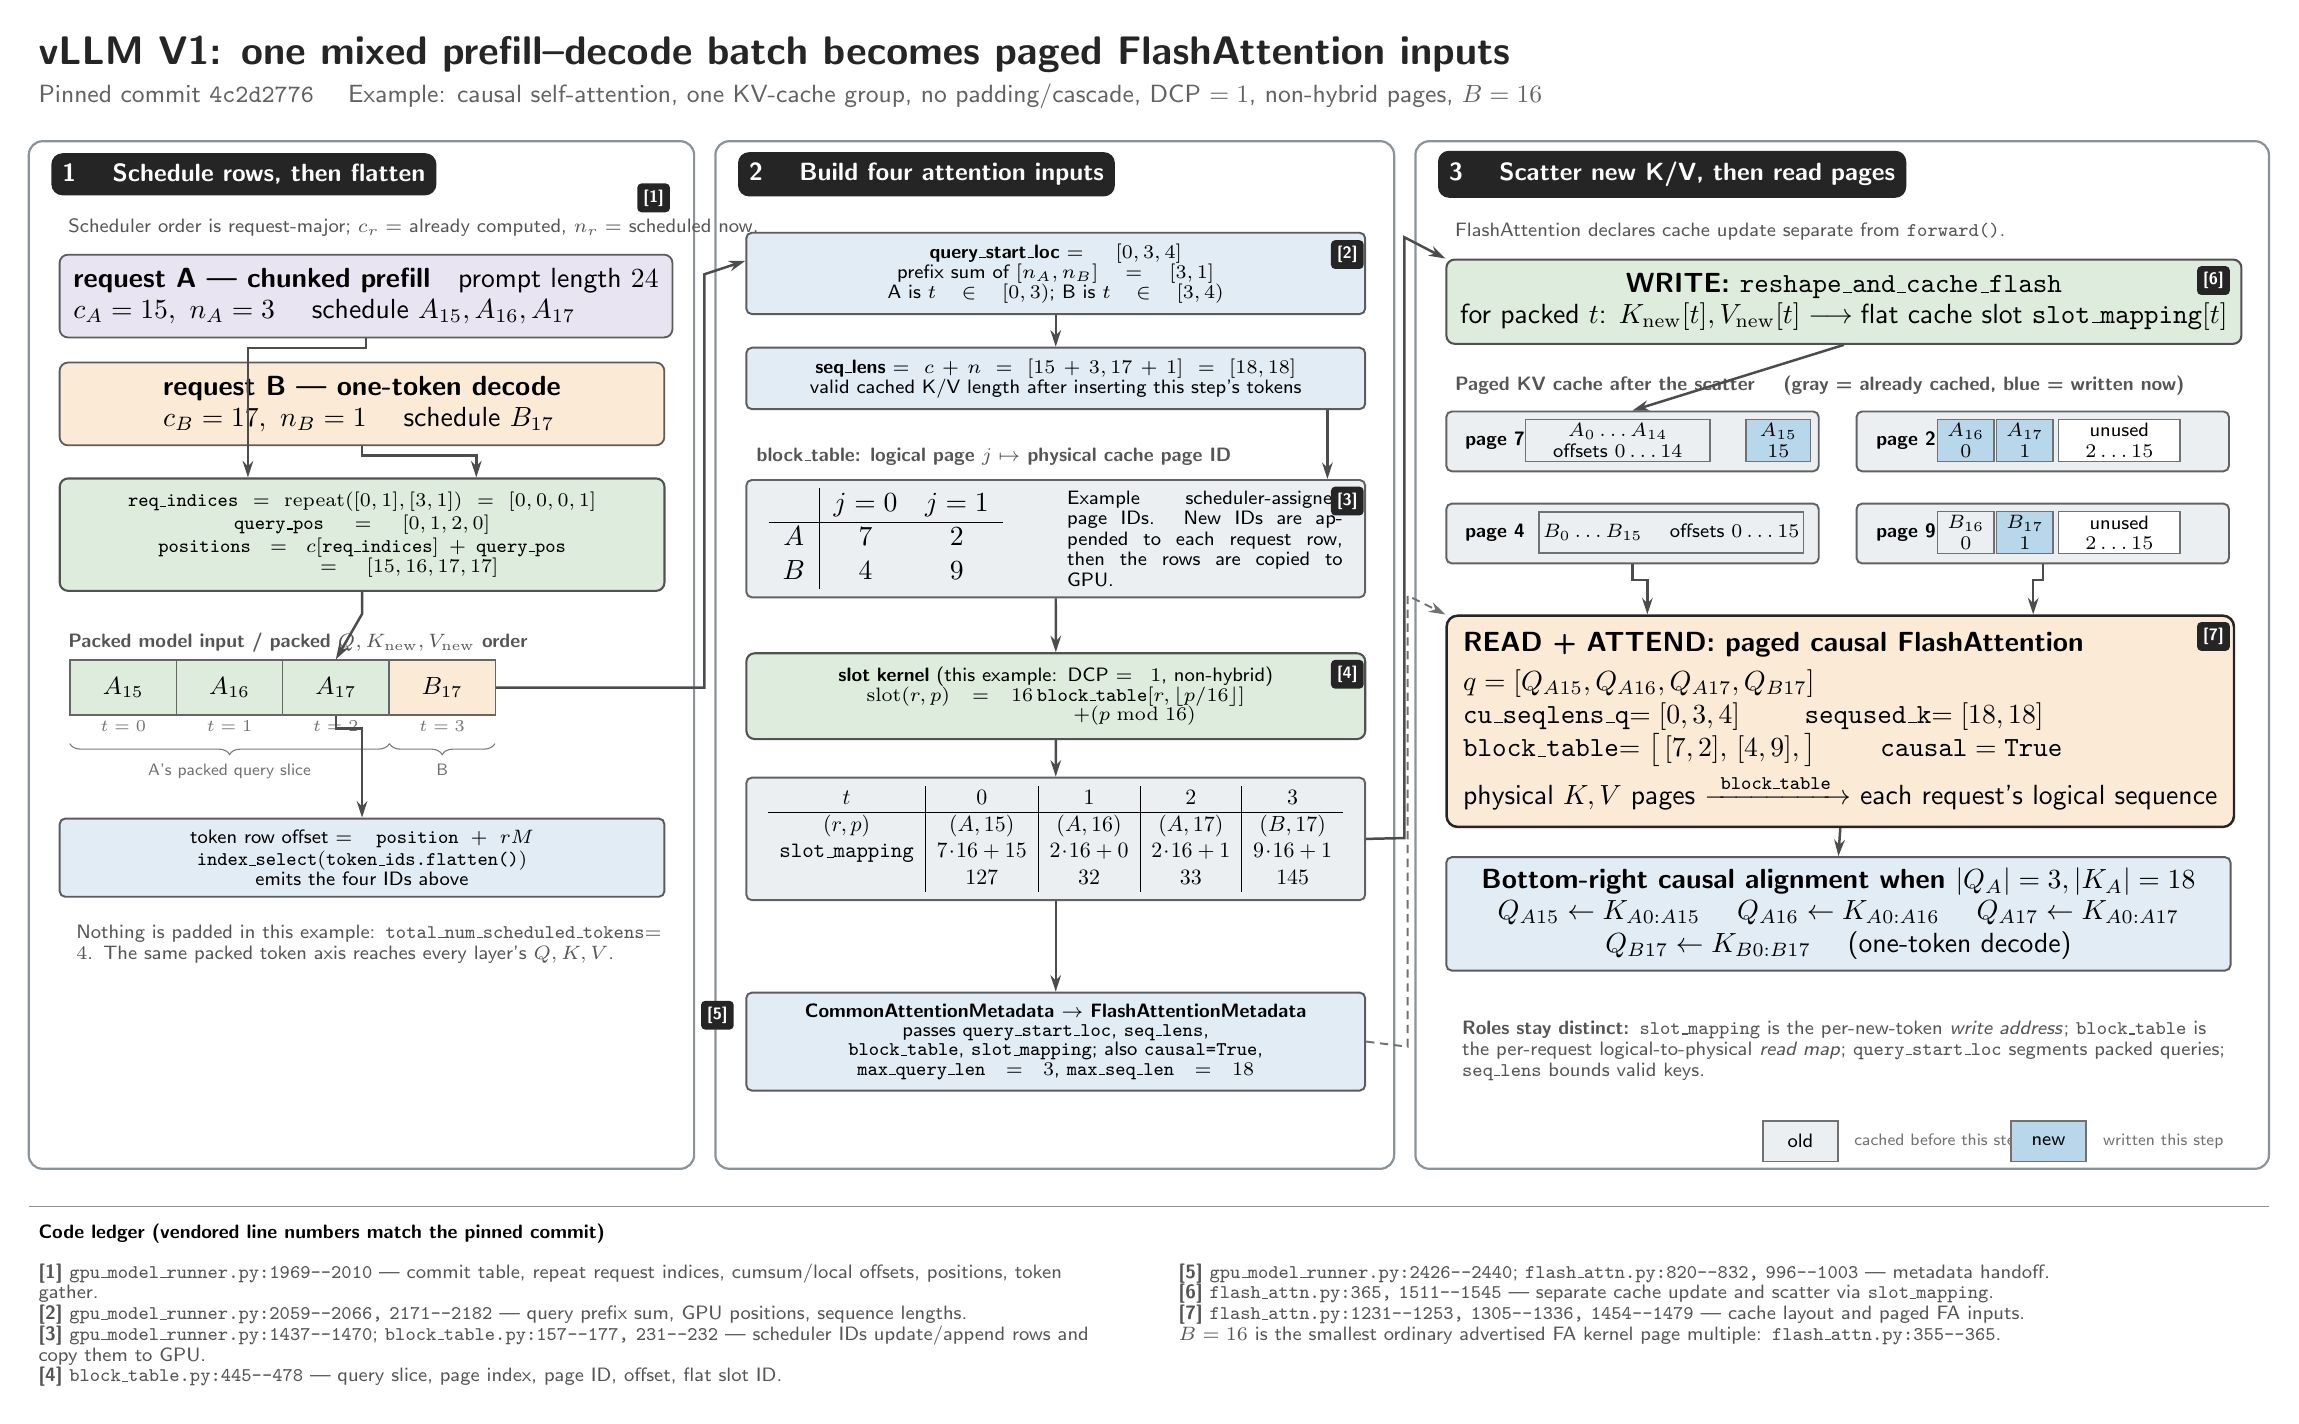
\begin{tikzpicture}[
  x=1cm,y=1cm,
  >={Stealth[length=2.1mm,width=1.35mm]},
  font=\sffamily,
  panel/.style={draw=rulegray,line width=.8pt,rounded corners=5pt,fill=white},
  panelhead/.style={rounded corners=4pt,fill=ink,text=white,font=\sffamily\bfseries\small,inner sep=4pt,anchor=west},
  card/.style={draw=ink!75,line width=.65pt,rounded corners=3pt,fill=paperlavender,align=left,inner sep=5pt},
  op/.style={draw=ink!80,line width=.75pt,rounded corners=3pt,fill=papergreen,align=center,inner sep=5pt},
  tensor/.style={draw=ink!75,line width=.7pt,rounded corners=2pt,fill=paperblue,align=center,inner sep=4pt},
  cache/.style={draw=ink!72,line width=.7pt,rounded corners=2pt,fill=cachegray,align=center,inner sep=3pt},
  fanode/.style={draw=ink,line width=.9pt,rounded corners=4pt,fill=paperpeach,align=left,inner sep=6pt},
  flow/.style={draw=ink!82,line width=.9pt,->},
  meta/.style={draw=ink!65,line width=.7pt,->,densely dashed},
  tinylabel/.style={font=\sffamily\fontsize{6.6}{7.5}\selectfont,text=ink!78,align=left},
  source/.style={font=\sffamily\bfseries\fontsize{6.3}{7}\selectfont,text=white,fill=ink,rounded corners=1.5pt,inner sep=2.2pt},
  index/.style={font=\sffamily\fontsize{6.2}{7}\selectfont,text=ink!65},
  cell/.style={draw=ink!70,line width=.55pt,minimum width=1.35cm,minimum height=.7cm,inner sep=1pt,font=\sffamily\small},
  slot/.style={draw=ink!65,line width=.55pt,minimum height=.52cm,inner sep=1.5pt,font=\sffamily\fontsize{6.7}{7.4}\selectfont,align=center}
]

% Title and scope.
\node[font=\sffamily\bfseries\Large,anchor=west,text=ink] at (0,15.35)
  {vLLM V1: one mixed prefill--decode batch becomes paged FlashAttention inputs};
\node[font=\sffamily\small,anchor=west,text=ink!72] at (0,14.82)
  {Pinned commit \texttt{4c2d2776} \quad Example: causal self-attention, one KV-cache group, no padding/cascade, DCP $=1$, non-hybrid pages, $B=16$};

% Main panel backgrounds.
\draw[panel] (0,1.20) rectangle (8.45,14.25);
\draw[panel] (8.72,1.20) rectangle (17.34,14.25);
\draw[panel] (17.61,1.20) rectangle (28.45,14.25);
\node[panelhead] at (.28,13.83) {1 \quad Schedule rows, then flatten};
\node[panelhead] at (9.00,13.83) {2 \quad Build four attention inputs};
\node[panelhead] at (17.89,13.83) {3 \quad Scatter new K/V, then read pages};

% PANEL 1: schedule and flatten.
\node[tinylabel,anchor=west] at (.38,13.15) {Scheduler order is request-major; $c_r=$ already computed, $n_r=$ scheduled now.};
\node[card,anchor=north west,minimum width=7.68cm] (reqA) at (.38,12.82) {
  \textbf{request A --- chunked prefill}\quad prompt length $24$\\[-1pt]
  $c_A=15,\ n_A=3$ \quad schedule $A_{15},A_{16},A_{17}$};
\node[card,fill=decode,anchor=north west,minimum width=7.68cm] (reqB) at (.38,11.45) {
  \textbf{request B --- one-token decode}\\[-1pt]
  $c_B=17,\ n_B=1$ \quad schedule $B_{17}$};
\node[source,anchor=north east] at (8.15,13.72) {[1]};

\node[op,anchor=north west,minimum width=7.68cm,text width=7.30cm,
      font=\sffamily\fontsize{7.2}{8.2}\selectfont] (flatten) at (.38,9.98) {
  $\texttt{req\_indices}=\operatorname{repeat}([0,1],[3,1])=[0,0,0,1]$\\
  $\texttt{query\_pos}=[0,1,2,0]$\\
  $\texttt{positions}=c[\texttt{req\_indices}]+\texttt{query\_pos}$\\[-1pt]
  $\hspace{1.2cm}=[15,16,17,17]$};

\node[tinylabel,anchor=west,font=\sffamily\bfseries\fontsize{7}{8}\selectfont] at (.38,7.88) {Packed model input / packed $Q,K_{\rm new},V_{\rm new}$ order};
\node[cell,fill=prefill] (t0) at (1.20,7.31) {$A_{15}$};
\node[cell,fill=prefill] (t1) at (2.55,7.31) {$A_{16}$};
\node[cell,fill=prefill] (t2) at (3.90,7.31) {$A_{17}$};
\node[cell,fill=decode]  (t3) at (5.25,7.31) {$B_{17}$};
\node[index] at (1.20,6.82) {$t=0$};
\node[index] at (2.55,6.82) {$t=1$};
\node[index] at (3.90,6.82) {$t=2$};
\node[index] at (5.25,6.82) {$t=3$};
\draw[decorate,decoration={brace,mirror,amplitude=4pt},draw=ink!60] (.52,6.60) -- (4.58,6.60)
  node[midway,below=4pt,index] {A's packed query slice};
\draw[decorate,decoration={brace,mirror,amplitude=4pt},draw=ink!60] (4.58,6.60) -- (5.92,6.60)
  node[midway,below=4pt,index] {B};

\node[tensor,anchor=north west,minimum width=7.68cm,text width=7.30cm,
      font=\sffamily\fontsize{7.2}{8.2}\selectfont] (gather) at (.38,5.66) {
  token row offset $=\texttt{position}+rM$\\
  $\texttt{index\_select}(\texttt{token\_ids.flatten()})$\\[-1pt]
  emits the four IDs above};
\node[tinylabel,anchor=north west,text width=7.45cm] at (.48,4.42) {
  Nothing is padded in this example: \texttt{total\_num\_scheduled\_tokens}$=4$.  The same packed token axis reaches every layer's $Q,K,V$.};

\draw[flow] (reqA.south) -- ++(0,-.12) -| ([xshift=-1.45cm]flatten.north);
\draw[flow] (reqB.south) -- ++(0,-.12) -| ([xshift=1.45cm]flatten.north);
\draw[flow] (flatten.south) -- ++(0,-.28) -- (t2.north);
\draw[flow] (t2.south) -- ++(0,-.16) -| (gather.north);

% PANEL 2: metadata construction.
\node[tensor,anchor=north west,minimum width=7.86cm,text width=7.46cm,
      font=\sffamily\fontsize{7.2}{8.2}\selectfont] (qsl) at (9.10,13.10) {
  \textbf{query\_start\_loc} $=[0,3,4]$\\[-1pt]
  prefix sum of $[n_A,n_B]=[3,1]$\\[-1pt]
  A is $t\in[0,3)$; B is $t\in[3,4)$};
\node[source,anchor=north east] at (16.96,13.00) {[2]};
\node[tensor,anchor=north west,minimum width=7.86cm,text width=7.46cm,
      font=\sffamily\fontsize{7.2}{8.2}\selectfont] (seqlens) at (9.10,11.64) {
  \textbf{seq\_lens} $=c+n=[15+3,17+1]=[18,18]$\\[-1pt]
  valid cached K/V length after inserting this step's tokens};

\node[tinylabel,anchor=west,font=\sffamily\bfseries\fontsize{7}{8}\selectfont] at (9.12,10.25)
  {block\_table: logical page $j \mapsto$ physical cache page ID};
\node[cache,anchor=north west,minimum width=7.86cm] (bt) at (9.10,9.96) {
  $\begin{array}{c|cc}
    &j=0&j=1\\ \hline
    A&7&2\\
    B&4&9
  \end{array}$
  \qquad \begin{minipage}{3.5cm}\fontsize{6.6}{7.4}\selectfont
  Example scheduler-assigned page IDs. New IDs are appended to each request row, then the rows are copied to GPU.
  \end{minipage}};
\node[source,anchor=north east] at (16.96,9.87) {[3]};

\node[op,anchor=north west,minimum width=7.86cm,text width=7.42cm,
      font=\sffamily\fontsize{7.0}{8.0}\selectfont] (slotop) at (9.10,7.76) {
  \textbf{slot kernel} (this example: DCP $=1$, non-hybrid)\\[-1pt]
  $\operatorname{slot}(r,p)=16\,\texttt{block\_table}\!\left[r,\left\lfloor p/16\right\rfloor\right]$\\[-1pt]
  $\hspace{2.0cm}+(p\bmod16)$};
\node[source,anchor=north east] at (16.96,7.67) {[4]};

\node[cache,anchor=north west,minimum width=7.86cm] (smap) at (9.10,6.18) {
  \resizebox{7.30cm}{!}{$\begin{array}{c|c|c|c|c}
  t&0&1&2&3\\ \hline
  (r,p)&(A,15)&(A,16)&(A,17)&(B,17)\\
  \texttt{slot\_mapping}&7\!\cdot\!16+15&2\!\cdot\!16+0&2\!\cdot\!16+1&9\!\cdot\!16+1\\
  &127&32&33&145
  \end{array}$}};

\node[tensor,anchor=north west,minimum width=7.86cm,text width=7.38cm,
      font=\sffamily\fontsize{7.0}{8.0}\selectfont] (metadata) at (9.10,3.45) {
  \textbf{CommonAttentionMetadata $\rightarrow$ FlashAttentionMetadata}\\[-1pt]
  passes \texttt{query\_start\_loc}, \texttt{seq\_lens},\\[-1pt]
  \texttt{block\_table}, \texttt{slot\_mapping}; also \texttt{causal=True},\\[-1pt]
  $\texttt{max\_query\_len}=3$, $\texttt{max\_seq\_len}=18$};
\node[source,anchor=north east] at (8.96,3.34) {[5]};

\draw[flow] (qsl.south) -- (seqlens.north);
\draw[flow] ([xshift=3.45cm]seqlens.south) -- ([xshift=3.45cm]bt.north);
\draw[flow] (bt.south) -- (slotop.north);
\draw[flow] (slotop.south) -- (smap.north);
\draw[flow] (smap.south) -- (metadata.north);
\draw[flow] (t3.east) -- (8.58,7.31) -- (8.58,12.56) -- ([yshift=.16cm]qsl.west);

% PANEL 3: backend cache update and attention read.
\node[tinylabel,anchor=west] at (17.99,13.10) {FlashAttention declares cache update separate from \texttt{forward()}.};
\node[op,anchor=north west,minimum width=9.96cm] (write) at (17.99,12.76) {
  \textbf{WRITE: \texttt{reshape\_and\_cache\_flash}}\\[-1pt]
  for packed $t$: $K_{\rm new}[t],V_{\rm new}[t]\longrightarrow\text{flat cache slot }\texttt{slot\_mapping}[t]$};
\node[source,anchor=north east] at (27.96,12.67) {[6]};

\node[tinylabel,anchor=west,font=\sffamily\bfseries\fontsize{7}{8}\selectfont] at (17.99,11.15)
  {Paged KV cache after the scatter \quad (gray = already cached, blue = written now)};

\node[cache,anchor=north west,minimum width=4.73cm,minimum height=.76cm] (p7) at (17.99,10.83) {};
\node[anchor=west,font=\sffamily\bfseries\fontsize{6.8}{7.4}\selectfont] at (18.12,10.45) {page 7};
\node[slot,fill=cachegray,minimum width=2.34cm] at (20.18,10.45) {$A_{0}\ldots A_{14}$\\ offsets $0\ldots14$};
\node[slot,fill=newblue,minimum width=.82cm] at (22.22,10.45) {$A_{15}$\\ $15$};

\node[cache,anchor=north west,minimum width=4.73cm,minimum height=.76cm] (p2) at (23.20,10.83) {};
\node[anchor=west,font=\sffamily\bfseries\fontsize{6.8}{7.4}\selectfont] at (23.34,10.45) {page 2};
\node[slot,fill=newblue,minimum width=.72cm] at (24.60,10.45) {$A_{16}$\\ $0$};
\node[slot,fill=newblue,minimum width=.72cm] at (25.35,10.45) {$A_{17}$\\ $1$};
\node[slot,fill=white,minimum width=1.54cm] at (26.55,10.45) {unused\\ $2\ldots15$};

\node[cache,anchor=north west,minimum width=4.73cm,minimum height=.76cm] (p4) at (17.99,9.66) {};
\node[anchor=west,font=\sffamily\bfseries\fontsize{6.8}{7.4}\selectfont] at (18.12,9.28) {page 4};
\node[slot,fill=cachegray,minimum width=3.18cm] at (20.86,9.28) {$B_{0}\ldots B_{15}$ \quad offsets $0\ldots15$};

\node[cache,anchor=north west,minimum width=4.73cm,minimum height=.76cm] (p9) at (23.20,9.66) {};
\node[anchor=west,font=\sffamily\bfseries\fontsize{6.8}{7.4}\selectfont] at (23.34,9.28) {page 9};
\node[slot,fill=cachegray,minimum width=.72cm] at (24.60,9.28) {$B_{16}$\\ $0$};
\node[slot,fill=newblue,minimum width=.72cm] at (25.35,9.28) {$B_{17}$\\ $1$};
\node[slot,fill=white,minimum width=1.54cm] at (26.55,9.28) {unused\\ $2\ldots15$};

\node[fanode,anchor=north west,minimum width=9.96cm] (faread) at (17.99,8.24) {
  \textbf{READ + ATTEND: paged causal FlashAttention}\\[2pt]
  $q=[Q_{A15},Q_{A16},Q_{A17},Q_{B17}]$\\
  \texttt{cu\_seqlens\_q}$=[0,3,4]$ \qquad \texttt{seqused\_k}$=[18,18]$\\
  \texttt{block\_table}$=\bigl[\,[7,2],\,[4,9],\bigr]$ \qquad $\texttt{causal}=\texttt{True}$\\[2pt]
  physical $K,V$ pages $\xrightarrow{\ \texttt{block\_table}\ }$ each request's logical sequence};
\node[source,anchor=north east] at (27.96,8.15) {[7]};

\node[tensor,anchor=north west,minimum width=9.96cm] (visible) at (17.99,5.17) {
  \textbf{Bottom-right causal alignment when $|Q_A|=3, |K_A|=18$}\\[-1pt]
  $Q_{A15}\leftarrow K_{A0:A15}$ \quad
  $Q_{A16}\leftarrow K_{A0:A16}$ \quad
  $Q_{A17}\leftarrow K_{A0:A17}$\\
  $Q_{B17}\leftarrow K_{B0:B17}$ \quad (one-token decode)};

\node[tinylabel,anchor=north west,text width=9.7cm] at (18.08,3.20) {
  \textbf{Roles stay distinct:} \texttt{slot\_mapping} is the per-new-token \emph{write address}; \texttt{block\_table} is the per-request logical-to-physical \emph{read map}; \texttt{query\_start\_loc} segments packed queries; \texttt{seq\_lens} bounds valid keys.};

\draw[flow] (write.south) -- (p7.north);
\draw[flow] (p4.south) -- ++(0,-.20) -| ([xshift=-2.45cm]faread.north);
\draw[flow] (p9.south) -- ++(0,-.20) -| ([xshift=2.45cm]faread.north);
\draw[flow] (faread.south) -- (visible.north);
\draw[flow] (smap.east) -- (17.47,5.40) -- (17.47,13.03) -- (write.north west);
\draw[meta] (metadata.east) -- (17.51,2.75) -- (17.51,8.48) -- (faread.north west);

% Source ledger: exact vendored code locations at the pinned commit.
\draw[draw=rulegray,line width=.55pt] (0,.72) -- (28.45,.72);
\node[font=\sffamily\bfseries\fontsize{7}{8}\selectfont,anchor=west] at (0,.38) {Code ledger (vendored line numbers match the pinned commit)};
\node[tinylabel,anchor=north west,text width=13.75cm] at (0,.12) {
  \textbf{[1]} \texttt{gpu\_model\_runner.py:1969--2010} --- commit table, repeat request indices, cumsum/local offsets, positions, token gather.\\
  \textbf{[2]} \texttt{gpu\_model\_runner.py:2059--2066, 2171--2182} --- query prefix sum, GPU positions, sequence lengths.\\
  \textbf{[3]} \texttt{gpu\_model\_runner.py:1437--1470}; \texttt{block\_table.py:157--177, 231--232} --- scheduler IDs update/append rows and copy them to GPU.\\
  \textbf{[4]} \texttt{block\_table.py:445--478} --- query slice, page index, page ID, offset, flat slot ID.};
\node[tinylabel,anchor=north west,text width=13.75cm] at (14.48,.12) {
  \textbf{[5]} \texttt{gpu\_model\_runner.py:2426--2440}; \texttt{flash\_attn.py:820--832, 996--1003} --- metadata handoff.\\
  \textbf{[6]} \texttt{flash\_attn.py:365, 1511--1545} --- separate cache update and scatter via \texttt{slot\_mapping}.\\
  \textbf{[7]} \texttt{flash\_attn.py:1231--1253, 1305--1336, 1454--1479} --- cache layout and paged FA inputs.\\
  $B=16$ is the smallest ordinary advertised FA kernel page multiple: \texttt{flash\_attn.py:355--365}.};

% Small semantic legend.
\node[slot,fill=cachegray,minimum width=.95cm] at (22.50,1.55) {old};
\node[index,anchor=west] at (23.06,1.55) {cached before this step};
\node[slot,fill=newblue,minimum width=.95cm] at (25.65,1.55) {new};
\node[index,anchor=west] at (26.22,1.55) {written this step};

\end{tikzpicture}
\end{document}
